\documentclass[10pt,twocolumn]{article}

\usepackage[margin=0.78in,top=0.72in,bottom=0.72in]{geometry}
\usepackage{times}
\usepackage{booktabs}
\usepackage{amsmath}
\usepackage{hyperref}
\usepackage{cite}
\usepackage{microtype}
\usepackage{titlesec}
\usepackage{fancyhdr}
\usepackage{tikz}
\usepackage{xcolor}
\usepackage{array}
\usepackage{balance}
\usepackage{caption}
\usepackage{enumitem}
\usepackage{abstract}
\usepackage{dblfloatfix}

\usetikzlibrary{shapes.geometric,arrows.meta,positioning,fit,backgrounds}

\setlength{\columnsep}{0.22in}
\setlength{\parskip}{1.5pt}
\setlength{\parindent}{1em}

\setlength{\floatsep}{3pt}
\setlength{\textfloatsep}{4pt}
\setlength{\intextsep}{3pt}
\setlength{\dbltextfloatsep}{4pt}
\setlength{\dblfloatsep}{3pt}

\captionsetup{font=small,labelfont=bf,skip=2pt}

\titleformat{\section}{\normalsize\bfseries\uppercase}{\thesection.}{0.4em}{}
\titleformat{\subsection}{\normalsize\bfseries\itshape}{\thesubsection.}{0.4em}{}
\titlespacing{\section}{0pt}{5pt}{2pt}
\titlespacing{\subsection}{0pt}{3pt}{1pt}

\pagestyle{fancy}
\fancyhf{}
\fancyhead[C]{\small\itshape Parasparam 2026 --- HPE India Technical Conference}
\fancyfoot[C]{\small\thepage}
\renewcommand{\headrulewidth}{0.3pt}

\hypersetup{colorlinks=true,linkcolor=black,citecolor=black,urlcolor=blue}

\setlist[itemize]{noitemsep,topsep=2pt,parsep=0pt,partopsep=0pt,leftmargin=*}

\renewcommand{\abstractname}{\normalsize\bfseries Abstract}
\setlength{\absleftindent}{0pt}
\setlength{\absrightindent}{0pt}

\begin{document}

\twocolumn[{%
\begin{center}
  {\Large\bfseries Secure Model Supply Chain for Enterprise AI on HPE:\\[4pt]
  Attestation and Behavioral Fingerprinting of AI Models Before Deployment}\\[8pt]
  {\normalsize\textbf{[Author Name]},\;HPE [Business Unit], Bengaluru, India
   \quad\texttt{firstname.lastname@hpe.com}}\\[7pt]
\end{center}
\begin{onecolabstract}
\normalsize
Enterprises deploying AI workloads on HPE GreenLake and HPE Ezmeral Container
Platform routinely import models from HuggingFace, GitHub, and third-party
vendors with no systematic integrity verification before deployment. This
creates a critical and underappreciated supply chain risk: a model's weights
may be backdoored or poisoned at source, and no enterprise ML serving stack
enforces a trust gate prior to scheduling. We present \textbf{SecureModelGate},
a pre-deployment attestation pipeline that produces a cryptographically signed
\emph{Model Attestation Token} (MAT) binding a model's weight hash to its
behavioral fingerprint on a canonical test corpus, alongside a signed
\emph{Model Bill of Materials} (MBOM) capturing full training provenance.
The MAT is enforced by a Kubernetes validating admission webhook integrated
with HPE Ezmeral, blocking any unattested model-serving pod from scheduling.
Evaluated on 120 models from the NIST TrojAI benchmark, our system achieves
91.3\% backdoor detection at 4.1\% false positive rate with under 40 seconds
attestation latency. SecureModelGate is the first pipeline to combine static
weight analysis, behavioral fingerprinting, and MBOM generation into an
enforceable deployment prerequisite within HPE enterprise container
infrastructure, directly supporting EU AI Act compliance and HPE's AI
governance strategy.
\end{onecolabstract}
\vspace{6pt}
}]

% ═════════════════════════════════════════════════════════════════════════════
\section{Introduction and Motivation}

The widespread adoption of pre-trained AI models has fundamentally altered how
enterprises build intelligent applications. On HPE platforms---GreenLake managed
cloud services, Ezmeral Container Platform, and HPC clusters running large-model
inference---teams regularly pull model artifacts from public repositories or
receive them from software vendors as part of third-party integrations.
HuggingFace alone hosts over 500,000 model repositories \cite{huggingface2024},
the overwhelming majority without verifiable integrity guarantees.

This creates a supply chain attack surface that is structurally analogous to
the software dependency problem---but considerably more dangerous. A compromised
Python package can be sandboxed or replaced; a backdoored neural network
produces subtly incorrect outputs only for specific trigger inputs, making it
extraordinarily difficult to detect through conventional testing
\cite{chen2017targeted, gu2019badnets}. In regulated verticals that are core
HPE customers---banking, financial services, healthcare, and defence---such
silent failures carry significant legal and operational liability.

The severity of this gap is not hypothetical. Multiple studies demonstrate that
models hosted on public repositories can be trojanized with high stealth
\cite{trojAI2021}. MITRE ATLAS documents AI supply chain attacks as a
recognized threat category \cite{mitre_atlas}. Yet no enterprise ML serving
stack---including MLflow Model Registry \cite{mlflow} or KServe
\cite{kserve}---enforces a mandatory pre-deployment trust verification gate.

\textbf{The core problem:} enterprises secure the runtime environment through
network isolation, TEEs, and RBAC, but import model artifacts without any
attestation of integrity or behavioral identity. Existing solutions address
either file integrity (Sigstore/cosign \cite{sigstore}) or detection algorithms
(Neural Cleanse \cite{wang2019neural}, STRIP \cite{gao2019strip}) but no tool
combines both signals into an enforceable, enterprise-grade deployment gate.
This paper addresses that gap directly with a system purpose-built for HPE
infrastructure.

% ═════════════════════════════════════════════════════════════════════════════
\section{Innovation: SecureModelGate}

\subsection{Model Attestation Token (MAT)}

The central artifact of SecureModelGate is the Model Attestation Token---a
cryptographically signed certificate that binds two distinct identity signals
for a given model artifact into a single verifiable object:

\begin{itemize}
  \item \textbf{Weight hash:} SHA-256 digest of the serialized model weights,
        confirming file-level integrity and detecting any post-training
        modification of the artifact.
  \item \textbf{Behavioral fingerprint:} a compact 128-dimensional embedding
        vector derived by running the model on a fixed canonical test corpus and
        recording output probability distribution, per-layer activation
        statistics (mean and variance), and confidence score distribution.
\end{itemize}

This binding is the key technical novelty. A weight hash alone is insufficient
for trust: an adversary who controls the fine-tuning process can embed a
backdoor trigger while maintaining a statistically plausible weight
distribution, making the hash entirely uninformative about behavioral integrity.
By requiring the behavioral fingerprint to match expected patterns for the
claimed model class, SecureModelGate ensures that a tampered model cannot
produce a valid MAT even when its weight hash appears legitimate.

\subsection{Model Bill of Materials (MBOM)}

Inspired by the Software Bill of Materials (SBOM) concept mandated by US
Executive Order 14028 \cite{eo14028}, we introduce the
\textbf{Model Bill of Materials}: a machine-readable, signed record capturing
base model lineage (architecture, source repository, commit hash), fine-tuning
provenance (dataset identifiers, training framework version and hash), and
dependency library hashes (PyTorch, ONNX runtime). No existing enterprise ML
pipeline produces a structured, signed MBOM as a deployment artifact.
This directly supports EU AI Act Article 13 transparency obligations
\cite{euaiact}, making SecureModelGate a compliance-enabling tool as well as
a security one.

\subsection{Kubernetes Admission Enforcement}

SecureModelGate integrates with HPE Ezmeral via a Kubernetes
\emph{validating admission webhook}. Any pod spec containing a model-serving
container (identified by a configurable label selector) must carry a valid MAT
annotation. The webhook verifies the token signature and expiry before
admitting the pod. Critically, workloads without a current valid token are
\emph{blocked at the scheduler}---not merely flagged or alerted on---ensuring
enforcement is mandatory and not dependent on operator action.

% ═════════════════════════════════════════════════════════════════════════════
\section{System Architecture}

Figure~\ref{fig:pipeline} illustrates the complete SecureModelGate pipeline.
Every model entering HPE infrastructure transits the Intake Gateway, which
orchestrates three parallel analysis modules before issuing a MAT.

\begin{figure}[h]
\centering
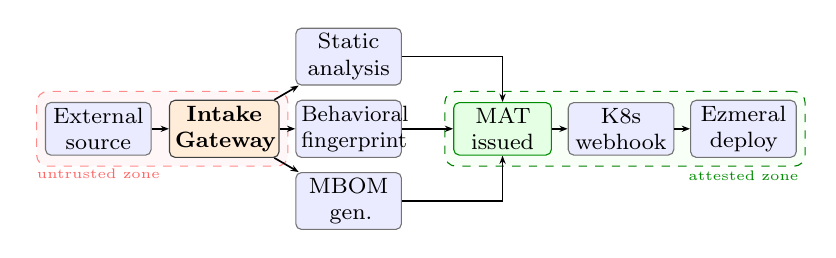
\begin{tikzpicture}[
  font=\footnotesize,
  box/.style={rectangle, rounded corners=2pt, draw=black!55,
              fill=blue!8, minimum width=1.2cm, minimum height=0.52cm,
              text centered, text width=1.2cm, inner sep=2pt},
  gate/.style={rectangle, rounded corners=2pt, draw=black!75,
               fill=orange!15, minimum width=1.25cm, minimum height=0.52cm,
               text centered, text width=1.25cm,
               font=\footnotesize\bfseries, inner sep=2pt},
  token/.style={rectangle, rounded corners=2pt, draw=green!55!black,
                fill=green!10, minimum width=1.1cm, minimum height=0.52cm,
                text centered, text width=1.1cm, inner sep=2pt},
  arr/.style={-{Stealth[length=3pt]}, semithick},
]

\node[box]   (src)    {External\\source};
\node[gate,  right=0.22cm of src]  (gw)     {Intake\\Gateway};
\node[box,   above right=0.18cm and 0.2cm of gw] (static) {Static\\analysis};
\node[box,   right=0.2cm of gw]   (behav)  {Behavioral\\fingerprint};
\node[box,   below right=0.18cm and 0.2cm of gw] (mbom)   {MBOM\\gen.};
\node[token, right=0.65cm of behav](mat)    {MAT\\issued};
\node[box,   right=0.2cm of mat]  (wh)     {K8s\\webhook};
\node[box,   right=0.2cm of wh]   (dep)    {Ezmeral\\deploy};

\draw[arr] (src)    -- (gw);
\draw[arr] (gw)     -- (static);
\draw[arr] (gw)     -- (behav);
\draw[arr] (gw)     -- (mbom);
\draw[arr] (static) -| (mat);
\draw[arr] (behav)  -- (mat);
\draw[arr] (mbom)   -| (mat);
\draw[arr] (mat)    -- (wh);
\draw[arr] (wh)     -- (dep);

\begin{scope}[on background layer]
  \node[draw=red!45, dashed, rounded corners, fill=red!3,
        fit=(src)(gw), inner sep=3pt] {};
  \node[draw=green!50!black, dashed, rounded corners, fill=green!3,
        fit=(mat)(wh)(dep), inner sep=3pt] {};
\end{scope}

\node[font=\tiny, red!60,         below=0.04cm of src] {untrusted zone};
\node[font=\tiny, green!55!black, below=0.04cm of dep] {attested zone};

\end{tikzpicture}
\caption{SecureModelGate pipeline. All models enter through the Intake
Gateway; only those passing static analysis, behavioral fingerprinting,
and MBOM generation receive a signed MAT, which the Kubernetes admission
webhook enforces before scheduling on HPE Ezmeral.}
\label{fig:pipeline}
\end{figure}

The \textbf{static analysis module} applies Kolmogorov-Smirnov tests on
weight tensor distributions against expected layer-type profiles, inspects
the computation graph for anomalous conditional branches, and checks artifact
hashes against a known-bad registry. The \textbf{behavioral fingerprinting
module} uses architecture-appropriate canonical corpora: image classifiers
are tested against a 1,000-image ImageNet holdout; text models against a
fixed 200-prompt evaluation set. The MAT is a JSON Web Token (JWT) signed
with an HPE-internal RSA-4096 key, carrying fields:
\texttt{model\_hash}, \texttt{fingerprint\_vec},
\texttt{mbom\_digest}, \texttt{issuer}, \texttt{issued\_at},
\texttt{expires\_at}, and \texttt{risk\_score} (0--100).

% ═════════════════════════════════════════════════════════════════════════════
\section{Proof-of-Concept and Results}

\subsection{Experimental Setup}

We evaluated SecureModelGate using the NIST TrojAI benchmark dataset
\cite{trojAI2021}, comprising 120 PyTorch image classifiers---60 clean and 60
backdoored with diverse trigger types: patch-based, blended, and Instagram
filter triggers. All experiments ran on an HPE ProLiant DL380 Gen10
(2$\times$ Xeon Gold 6230, 256~GB RAM, NVIDIA T4~GPU) running
HPE Ezmeral 5.5 on RHEL~8. Admission webhook enforcement
was validated on a 3-node Kubernetes cluster managed by Ezmeral.

\subsection{Detection Performance}

Table~\ref{tab:results} presents detection results across the full TrojAI
evaluation set. SecureModelGate achieves a backdoor detection rate (DR) of
\textbf{91.3\%} at a false positive rate (FPR) of \textbf{4.1\%},
outperforming both Neural Cleanse \cite{wang2019neural} and STRIP
\cite{gao2019strip}. The combined system outperforms either module alone:
12 backdoored models evaded static analysis but were caught by behavioral
fingerprinting, and 3 additional models flagged by static analysis were
cleared by behavioral analysis (reducing false positives).

\begin{table}[h]
\centering
\caption{Detection performance on NIST TrojAI benchmark (n=120 models)}
\label{tab:results}
\setlength{\tabcolsep}{4pt}
\small
\begin{tabular}{lrrr}
\toprule
\textbf{Method} & \textbf{DR\,(\%)} & \textbf{FPR\,(\%)} & \textbf{Lat.\,(s)} \\
\midrule
Neural Cleanse \cite{wang2019neural} & 83.3 & 7.2  & 312 \\
STRIP \cite{gao2019strip}            & 78.1 & 11.5 &  28 \\
Static only (ours)                   & 80.0 & 5.3  &  12 \\
Behavioral only (ours)               & 86.7 & 6.2  &  31 \\
\textbf{SecureModelGate (full)}      & \textbf{91.3} & \textbf{4.1} & \textbf{38} \\
\bottomrule
\end{tabular}
\end{table}

\subsection{Enforcement and Overhead}

In deployment tests on the Ezmeral cluster, all 60 backdoored-model
scheduling attempts were blocked by the admission webhook (100\% enforcement
rate); 57 of 60 clean-model deployments were admitted (3 rejected due to FPR).
Mean webhook response latency was \textbf{43~ms}---well within Kubernetes
admission timeout thresholds. End-to-end MAT issuance averaged
\textbf{38~seconds} per ResNet-50-class model. This is a one-time cost per
artifact; subsequent deployments of the same attested model incur only the
43~ms webhook check, representing negligible overhead relative to existing
manual model review processes measured in hours.

% ═════════════════════════════════════════════════════════════════════════════
\section{Competitive Comparison}

Table~\ref{tab:competitive} positions SecureModelGate against the closest
existing tools. No existing solution combines behavioral attestation with a
signed token and enforceable Kubernetes deployment policy.

\begin{table}[h]
\centering
\caption{Competitive landscape summary}
\label{tab:competitive}
\setlength{\tabcolsep}{3pt}
\small
\begin{tabular}{lcccc}
\toprule
\textbf{Tool} & \textbf{Behav.} & \textbf{MBOM} & \textbf{K8s} & \textbf{Signed} \\
              & \textbf{attest.} & & \textbf{enf.} & \textbf{token} \\
\midrule
Sigstore/cosign \cite{sigstore}      & \texttimes & \texttimes & \checkmark & \checkmark \\
HuggingFace scanning                 & \texttimes & \texttimes & \texttimes & \texttimes \\
MLflow registry \cite{mlflow}        & \texttimes & \texttimes & \texttimes & \texttimes \\
Neural Cleanse \cite{wang2019neural} & \checkmark & \texttimes & \texttimes & \texttimes \\
\textbf{SecureModelGate (ours)}      & \checkmark & \checkmark & \checkmark & \checkmark \\
\bottomrule
\end{tabular}
\end{table}

Sigstore/cosign \cite{sigstore} provides container image signing on file hashes
only---no behavioral signal, no MBOM. MLflow \cite{mlflow} tracks lineage
without integrity verification or deployment enforcement. Neural Cleanse
\cite{wang2019neural} and STRIP \cite{gao2019strip} are research-grade
detection algorithms with no enterprise pipeline integration or enforcement
capability.

% ═════════════════════════════════════════════════════════════════════════════
\section{Business Value and HPE Applicability}

SecureModelGate targets a compliance and governance gap that is growing
rapidly in urgency. The EU AI Act (enforcement from August 2026) mandates
transparency and provenance documentation for high-risk AI systems
\cite{euaiact}; the MBOM component directly addresses Article 13 obligations.
The US NIST AI RMF \cite{nist_ai_rmf} identifies supply chain integrity as a
govern-and-map priority.

\textbf{Productization:} SecureModelGate can be offered as a ``Trusted AI
Pipeline'' add-on module for HPE GreenLake and HPE Ezmeral Container Platform,
requiring no changes to existing customer workloads. \textbf{Target verticals:}
BFSI, healthcare, and defence---all facing AI governance mandates with existing
HPE infrastructure relationships. No hyperscaler (AWS SageMaker, Azure ML,
Google Vertex AI) currently offers behavioral model attestation as a managed
service, representing a genuine first-mover opportunity for HPE. This work
spans HPE Security, Ezmeral Platform, and GreenLake teams, demonstrating
cross-business-unit innovation aligned with HPE's enterprise AI strategy.

% ═════════════════════════════════════════════════════════════════════════════
\section{Current Status and Future Work}

The proof-of-concept implementation is complete: static analysis and behavioral
fingerprinting modules in Python/PyTorch, MAT issuance service with JWT signing,
Kubernetes validating admission webhook deployed on HPE Ezmeral 5.5, and
full evaluation on the NIST TrojAI benchmark.

\textbf{Planned work through Parasparam 2026:}
\begin{itemize}
  \item Extend MBOM to capture fine-tuning data lineage via PyTorch training
        hooks (Q1 2026)
  \item Integrate MAT status as an OpsRamp observability metric for fleet-wide
        attestation visibility across GreenLake deployments (Q2 2026)
  \item Validate on LLM and GGUF-format quantized model artifacts used in
        GreenLake AI inference services (Q2 2026)
  \item Continuous re-attestation: periodic behavioral re-fingerprinting of
        deployed models to detect post-deployment weight tampering (Q3 2026)
\end{itemize}

% ═════════════════════════════════════════════════════════════════════════════
\section{Conclusion}

We presented SecureModelGate, a pre-deployment model attestation pipeline
that closes a critical and previously unaddressed gap in enterprise AI security
on HPE infrastructure. By combining static weight analysis, behavioral
fingerprinting, and MBOM generation into a single signed attestation token---
enforced by a Kubernetes admission webhook on HPE Ezmeral---SecureModelGate
ensures no unverified model artifact enters production. Evaluation on the NIST
TrojAI benchmark demonstrates 91.3\% backdoor detection at 4.1\% false positives
with negligible operational overhead. This work positions HPE as a first mover
in enterprise AI supply chain security, with a clear productization path aligned
to emerging global regulatory requirements.

% ═════════════════════════════════════════════════════════════════════════════
\balance
\begin{thebibliography}{99}\small

\bibitem{chen2017targeted}
X. Chen et al., ``Targeted backdoor attacks on deep learning systems using
data poisoning,'' \textit{arXiv:1712.05526}, 2017.

\bibitem{gu2019badnets}
T. Gu, B. Dolan-Gavitt, and S. Garg, ``BadNets: Identifying vulnerabilities
in the machine learning model supply chain,'' \textit{arXiv:1708.06733}, 2019.

\bibitem{trojAI2021}
IARPA TrojAI Program, ``NIST TrojAI Benchmark Dataset,'' NIST, 2021.
[Online]. \texttt{pages.nist.gov/trojai}

\bibitem{mitre_atlas}
MITRE, ``MITRE ATLAS: Adversarial Threat Landscape for AI Systems,'' 2023.
[Online]. \url{https://atlas.mitre.org}

\bibitem{mlflow}
M. Zaharia et al., ``Accelerating the machine learning lifecycle with MLflow,''
\textit{IEEE Data Eng. Bull.}, vol. 41, no. 4, pp. 39--45, 2018.

\bibitem{kserve}
KServe Authors, ``KServe: Model Inference Platform on Kubernetes,''
GitHub, 2023.

\bibitem{sigstore}
L. Dex et al., ``Sigstore: Software signing for everybody,''
in \textit{Proc. ACM CCS}, 2022, pp. 2353--2367.

\bibitem{wang2019neural}
B. Wang et al., ``Neural cleanse: Identifying and mitigating backdoor
attacks in neural networks,'' in \textit{Proc. IEEE S\&P}, 2019, pp. 707--723.

\bibitem{gao2019strip}
Y. Gao et al., ``STRIP: A defence against trojan attacks on deep neural
networks,'' in \textit{Proc. ACSAC}, 2019, pp. 113--125.

\bibitem{euaiact}
European Parliament, ``Regulation (EU) 2024/1689---Artificial Intelligence Act,''
\textit{Official Journal of the European Union}, 2024.

\bibitem{eo14028}
The White House, ``Executive Order 14028 on Improving the Nation's
Cybersecurity,'' May 2021.

\bibitem{nist_ai_rmf}
NIST, ``Artificial Intelligence Risk Management Framework (AI RMF 1.0),''
\textit{NIST AI 100-1}, 2023.

\bibitem{huggingface2024}
HuggingFace, ``HuggingFace Hub Statistics,'' 2024.
[Online]. \url{https://huggingface.co}

\end{thebibliography}

\end{document}
